\iffalse

%%%%%%%%%%%%%%%%%%%%%%%%%%%%%%%%%%%%%%%%%%%%%%%%%%%%%%%%%%%%%%%%%%%%%%%%
%
% This is the template file for the 6th International conference
% NONLINEAR ANALYSIS AND EXTREMAL PROBLEMS
% June 25-30, 2018
% Irkutsk, Russia
%
%%%%%%%%%%%%%%%%%%%%%%%%%%%%%%%%%%%%%%%%%%%%%%%%%%%%%%%%%%%%%%%%%%%%%%%%
% The preparation of the article is based on the standard llncs class
% (Lecture Notes in Computer Sciences), which is adjusted with style
% file of the conference.
%
% There are two ways of compilation of the file into PDF
% 1. Use pdfLaTeX (pdflatex), (LaTeX+DVIPS will not work);
% 2. Use LuaLaTeX (XeLaTeX will work too).
% When using LuaLaTeX You will need TTF or OTF CMU fonts
% (Computer Modern Unicode). The fonts are installed with 'cm-unicode' package in
% a distribution of LaTeX % (https://www.ctan.org/tex-archive/fonts/cm-unicode),
% either by downloading and installing these fonts system wide, the address of their page is
% http://canopus.iacp.dvo.ru/%7Epanov/cm-unicode/
% The second option won't work in XeLaTeX.
%
% For MiKTeX (LaTeX distribution for Windows),
%  1. Package 'cm-unicode' is installed manually with the MiKTeX administration Console.
%  2. For the compilation of this example, namely, the stub figure, one will also need to
% download package 'pgf' manually. This package uses in the popular
% package tikz.
%  3. Tests showed that the rest of the required packages MiKTeX loads automatically (if
%     it is allowed). The 'auto download' option is
%     configured in 'Settings' section in MiKTeX Console.
%
%
% The easiest way to compile an article is to use pdfLaTeX, but
% the final layout of the book will be compiled with LuaLaTeX,
% as a result will be of better quality thanks to the package 'microtype' and
% use vector OTF instead of standard raster fonts of pdfLaTeX.
%
% In the case of questions and problems with the article compilation,
% write letters to e-mail: eugeneai@irnok.net, Cherkashin Evgeny.
%
% New version of the correcting style file will be available at the website:
%     https://github.com/eugeneai/nla-style
%     file - nla.sty
%
% Further instructions are in the text body of the template. The template itself
% is an article example.
%
% The LaTeX2e format is used!

% 12 points font size is used.
\documentclass[12pt]{llncs}

% The correcting style file is added.
\usepackage{todonotes}

\usepackage{nla} % This package is needed for compiling
                 % this template, it should be removed
                 % from your article.

% Many popular packages (amsXXX, graphicx, etc.) are already imported in the style file.
% If there is a conflict with your packages, try disabling them and compile
% the text.
%
% It would be convenient in the layout of the proceedings if the file names
% of the figures of different authors do not clash.
% To minimize the clash, the drawings can be placed in a separate subfolder
% named after the author or the title of the paper.
%
% \graphicspath{{ivanov-petrov-pics/}} % specifies the folder with images in png, pdf formats.
% or
% \graphicspath{{great-problem-solving-paper-pics/}}.

\begin{document}

% Text should be formatted in accordance with the 'article' class, using extensions like
% AMS.
%

\fi

\title{Bright Solitons in a (2+1)-dimensional Oceanic Model: Dynamics, Interaction and Molecule Formation\thanks{The research is supported through Young Scientist Training (YST) project by APCTP.}}
% First author
\author{Sakkaravarthi Karuppaiya}
\institute{Young Scientist Training Program, Asia-Pacific Center for Theoretical Physics (APCTP),\\ POSTECH Campus, Pohang – 37673, Republic of Korea\\
  \email{ksakkaravarthi@gmail.com}}
% etc

\maketitle

\begin{abstract}
In this work, we consider the following integrable (2+1)-dimensional nonlinear model which arises in different perspectives to describe the dynamics of ion acoustic waves in a magnetized plasma, deep water oceanic rogue waves, optical wave propagation in Erbium-doped coherently excited waveguides, Bragg grating optical fiber, etc.:\\
	{$~~\hspace{3.5cm} iq_t+aq_{xy}+2ib(qq_x^*-q^*q_x)q=0, $}\\
	where $q(x,y,t)$ is envelope of the wave, $x$ and $y$ are spatial variables while $t$ denotes the temporal variable and the symbol $*$ represents the complex conjugate. Here the coefficients $a$ and $b$ correspond to the dispersion and nonlinearity. 
	The above model can also be viewed as a (2+1)D extension of the standard (1+1)D focusing nonlinear Schr\"{o}dinger equation which appear in diverse fields of physics and show promising characteristics.    
	First, we construct bright soliton solutions by using the powerful bilinearization method and explore their propagation characteristics. Next, we investigate the interaction dynamics of bright solitons for different choices of parameters which show head-on and oblique type elastic interactions where the solitons reappear unaltered after interaction and exhibits only a phase-shift with explicit asymptotic analysis. Finally, we unravel the possibility of soliton molecule formation through velocity resonance mechanism which gives rise to the generation of breathers. Especially, we discuss the influence of dispersion and nonlinearities in the dynamics, interaction and molecules. The obtained results will add significant knowledge to the understanding of higher dimensional solitons. 

\keywords{Nonlinear Waves, Higher-dimensional Nonlinear Model, Bright Solitons, Interaction Dynamics, Soliton Molecules }
\end{abstract} \vspace{-0.75cm}
\begin{figure}[h]
  \centering 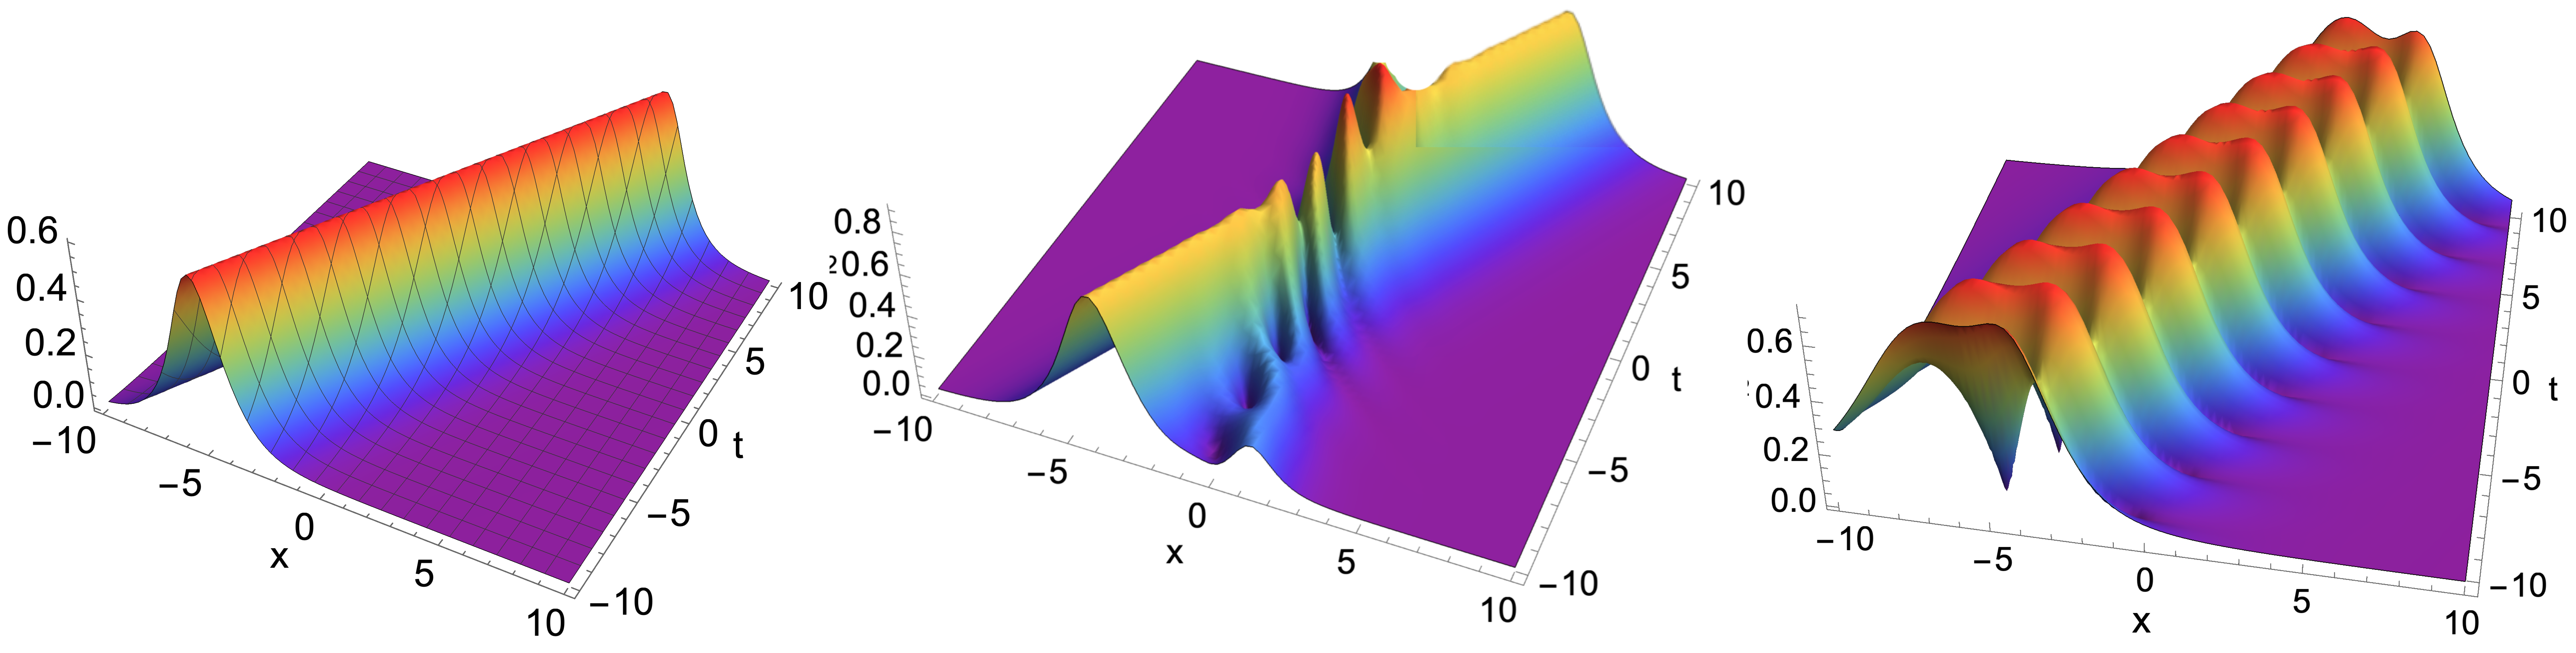
\includegraphics[width=0.9270\linewidth]{figure-Sakkaravarthi.png} 
  \caption{The dynamics of (a) single bright soliton, (b) two-soliton elastic interaction, (c) soliton molecule leading to breather formation.}\label{fig:example}
\end{figure}

%\noindent {\small Acknowledgment: The research is supported through Young Scientist Training (YST) project by APCTP.}

%\end{document}

